\chapter{Background}\label{first-c}
\section{Architettura di \textsc{Vampire}}
L'\emph{automated theorem prover} \textsc{Vampire} ha un'architettura complessa ma, analizzandola ad alto livello, è possibile riconoscere tre moduli 
principali:
\begin{enumerate}
    \item \emph{parser}
    \item \emph{preprocessor}
    \item \emph{kernel}
\end{enumerate}
\begin{figure}[H]
    \incfig{architettura}
\end{figure}


\subsection{Parser}
Il \emph{parser} è un modulo che permette la lettura di un problema da un file e la conseguente incapsulazione in una classe specifica.
Nel caso di un problema di logica del primo ordine con sintassi TPTP, viene diviso in più unità.
Ogni unità è una formula o una clausola a cui viene assegnato uno specifico tag in base al tipo (ipotesi, assioma, congettura, teorema, \dots).

Nel codice sorgente sono presenti le classi \verb|Problem|, \verb|Unit|, \verb|Formula|, \verb|Clause| e sono in relazione tra loro come mostrato nella figura \ref{fig:relazioni-classi}.
L'attributo \emph{kind} della classe \verb|Unit| permette la distinzione tra \verb|Clause| e \verb|Formula|.
Sono presenti altre classi, non rappresentate nella figura, che ereditano \verb|Formula| come:
\verb|AtomicFormula|, \verb|JunctionFormula|, \verb|BinaryFormula|, \dots 
\vspace{.3cm}
\begin{figure}[H]
    \begin{tikzpicture}
        \begin{class}{Problem}{-5,0}
            \attribute{- units : UnitList*}
        \end{class}
        \begin{class}{Unit}{-5,-2}
            \attribute{- kind : enum}
            \operation{+ getFormula()}
            \operation{+ asClause()}
        \end{class}
        \begin{class}{Formula}{-10,-5}
        \end{class}
        \begin{class}{Clause}{0,-5}
        \end{class}
        \begin{class}{QuantifiedFormula}{-10,-8}
            \inherit{Formula}
        \end{class}
        \begin{class}{NegatedFormula}{-4,-8}
            \inherit{Formula}
        \end{class}
    
        \unidirectionalAssociation{Problem}{}{}{Unit}
        \unidirectionalAssociation{Unit}{}{}{Formula}
        \unidirectionalAssociation{Unit}{}{}{Clause}
    \end{tikzpicture}
    \caption{Relazioni tra le classi per definire un problema}
    \label{fig:relazioni-classi}
\end{figure}
\subsection{Preprocessor}\label{sec-prepro}
Il \emph{\emph{preprocessor}} è un modulo che processa il problema in modo che sia trattabile dal \emph{kernel} in fase di risoluzione.
Per questo modulo è possibile abilitare numerose opzioni, inoltre vengono eseguite semplificazioni in modo da rendere il sistema il 
più veloce possibile. Di seguito sono descritti solo i passaggi fondamentali del \emph{preprocessing} \cite{reger2016new}: 
\begin{description}
    \item[I step] \emph{Rectify}: Il \emph{preprocessor} verifica se una formula ha variabili libere. Se la formula è aperta, 
    allora genera dei quantificatori per vincolare le variabili libere. Inoltre, verifica che per ogni variabile $x$ ci sia una sola occorrenza di $\exists x$ o $\forall x$. 
    \item[II step] \emph{Simplify}: Il \emph{preprocessor} verifica se una formula contiene $\top$ o $\bot$. Nel caso la formula contenesse uno dei due, allora
    viene semplificata.
    \item[III step] \emph{Flatten}: Il \emph{preprocessor} trasforma le formule in modo da renderle uniformi. Questo è solo uno step di formattazione che verrà eseguito più volte nel corso del preprocessing.
    \item[IV step] \emph{Unused definitions and pure predicate removal}: Il \emph{preprocessor} rimuove i predicati e le definizioni delle funzioni che non vengono usati.
    \item[V step] \emph{ENNF}: Il \emph{preprocessor} trasforma le formula in \emph{extended negative normal form}.
    \begin{definition}
        Una formula è in \emph{extended negation normal form} se non contiene $\rightarrow$, e tutte le $\neg$ sono spostate, il più possibile, verso l'interno.  
    \end{definition}
    \item[VI step] \emph{Naming}: Il \emph{preprocessor} definisce un nuovo predicato $p$ che viene usato come nome di una sotto-formula. 
    Questa tecnica viene utilizzata per evitare di generare un numero esponenziale di clausole nei prossimi passaggi di preprocessing.
    \begin{definition}
        Sia $\varphi|_\pi$ sotto-formula di $\varphi$ in posizione $\pi$ con variabili libere $\bar{x}$, allora si sostituisce $\varphi|_\pi$ con $p(\bar{x})$
        nuovo predicato e viene aggiunta la definizione $\text{def}(\varphi,\pi,p)$ tale che
        \[\text{def}(\varphi,\pi,p)=\begin{cases}
            \forall \bar{x} (p(\bar{x})\rightarrow \varphi|_\pi) & \text{se pol}(\varphi,\pi)=1\\
            \forall \bar{x} (\varphi|_\pi\rightarrow p(\bar{x})) & \text{se pol}(\varphi,\pi)=-1\\
            \forall \bar{x} (p(\bar{x})\leftrightarrow \varphi|_\pi) & \text{se pol}(\varphi,\pi)=0\\
        \end{cases}\]
        in cui $\text{pol}(\varphi,\pi)$ indica la polarità della sotto-formula di $\varphi$ in posizione $\pi$. $\text{pol}(\varphi,\pi)=0$ si verifica quando il simbolo di livello superiore di $\varphi|_\pi$ è 
        $\leftrightarrow$ o $\otimes$.   
    \end{definition}
    Questa tecnica viene adottata solo se il numero di clausole generate supera una certa soglia. Infatti, in 
    \textsc{Vampire}, nella classe \verb|Naming|, è presente un attributo \emph{threshold} che indica proprio questo limite.
    \item[VII step] \emph{NNF}: Il \emph{preprocessor} trasforma le formule in \emph{negation normal form}.
    \begin{definition}
        Una formula è in \emph{negation normal form} se non contiene $\rightarrow,\leftrightarrow,\otimes$, e tutte le $\neg$ sono spostate, il più possibile, verso l'interno.
    \end{definition}
    \item[VIII step] \emph{Skolemization}: Il \emph{preprocessor} applica questa tecnica per eliminare i $\exists$ dalle formule.
    \begin{definition}
        Sia $F=\exists x\mid\varphi(y_1,\dots,y_n,x)$ formula in negation normal form allora la \emph{skolemization} si ottiene tramite la seguente sostituzione:
        \[F=\exists x\mid\varphi(y_1,\dots,y_n,x)\Rightarrow F'=\varphi(y_1,\dots,y_n,x)\{x \mapsto sk(y_1,\dots,y_n)\}\]
        in cui $\{x \mapsto sk(y_1,\dots,y_n)\}$ indica che $x$, la variabile precedentemente vincolata dal quantificatore esistenziale nella formula $F$, 
        è sostituita da una nuova funzione $sk(y_1,\dots,y_n)$, detta di Skolem, nella formula $F'$.
    \end{definition}
    \item[IX step] \emph{Clausification}: Il \emph{preprocessor} trasforma tutte le formule in modo da ottenere 
    un insieme di clausole.
    \begin{definition}
        La \emph{clausification} è il risultato di:
        \begin{enumerate}
            \item $\forall x\mid\varphi(y_1,\dots,y_n,x)\Rightarrow\varphi(y_1,\dots,y_n,x)\{x \mapsto X\}$  in cui $X$ è una variabile designata che non occorre in $\varphi$
            \item Se una formula $F=\varphi'\land\varphi''$ allora viene spezzata in due unità diverse 
            $F'=\varphi'$ e $F''=\varphi''$
        \end{enumerate}
    \end{definition}  
\end{description} 
Alla fine di questi step, l'insieme di clausole risultanti è pronto per essere passato all'algoritmo di \emph{resolution}.
\subsection{Kernel}\label{sec-kernel}
Il \emph{kernel} è il sotto-sistema adibito alla risoluzione del problema. Per raggiungere questo obiettivo, 
viene implementato un algoritmo di saturazione che permette di trovare una confutazione all'insieme di clausole.
\'E possibile trovare la confutazione all'insieme tramite la sua saturazione con tutte le inferenze presenti nel calcolo. 
\textsc{Vampire} possiede numerose inferenze ma è possibile sceglierne un sottoinsieme e definire un sistema 
d'inferenze per la logica del primo ordine.

Formalmente, per definire un sistema d'inferenze bisogna prima definire un \emph{simplification ordering} e una funzione di selezione \cite{kovacs2013first,riazanov2002design}.
\begin{definition}
    Un ordinamento $\succ$ sui termini è detto \emph{simplification ordering} se rispetta le seguenti condizioni:
    \begin{enumerate}
        \item $\succ$ è \emph{ben formato} ovvero non esiste una sequenza infinita $t_0,t_1, \dots \text{tale che } t_0 \succ t_1 \succ \dots$
        \item $\succ$ è \emph{monotona} ovvero $l \succ r \rightarrow s(l)\succ s(r)$ per tutti i termini $s,l,r$
        \item $\succ$ è \emph{stabile} per la sostituzione ovvero $l \succ r \rightarrow l\theta \succ r\theta$
        \item $\succ$ ha la \emph{subterm property} ovvero se $r$ è sottotermine di $l$ e $l\neq r$ allora $l\succ r$   
    \end{enumerate}
\end{definition}
Questa definizione è estendibile agli atomi, ai letterali e alle clausole.
\begin{definition}
    Una funzione di selezione sceglie un sottoinsieme non vuoto di letterali in ogni clausola non vuota. In $\underline{L}\lor R$, \underline{L} indica il letterale selezionato.
\end{definition}
Il sistema di inferenze che viene definito di seguito è detto \emph{superposition inference system}.
\begin{definition}\label{supdef}
    Il \emph{superposition inference system} è un sistema di inferenze composto dalle seguenti regole:
    \begin{itemize}
        \item \textbf{Resolution}
        \begin{equation}\label{res-eq}
            \begin{gathered}
                \underline{\underline{A} \lor C_1 \quad\underline{\lnot A'}\lor C_2}\\
                (C_1 \lor C_2)\theta
            \end{gathered}
        \end{equation}
        in cui $\theta$ è l'unificatore più generale di $A$ e $A'$.
        \item \textbf{Factoring}\label{fact-eq}
        \begin{equation}
            \begin{gathered}
                \underline{\underline{A} \lor \underline{A'} \lor C}\\
                (A \lor C)\theta
            \end{gathered}
        \end{equation}
        in cui $\theta$ è l'unificatore più generale di $A$ e $A'$.
        \item \textbf{Superposition}
        \begin{equation}
            \begin{gathered}
                \underline{\underline{l=r} \lor C_1 \quad \underline{L[s]}\lor C_2} \quad \underline{\underline{l=r} \lor C_1 \quad \underline{t[s]=t'}\lor C_2} \quad \underline{\underline{l=r} \lor C_1 \quad \underline{t[s]\neq t'}\lor C_2}\\
                (L[r] \lor C_1 \lor C_2)\theta \qquad (t[r]=t' \lor C_1 \lor C_2)\theta \qquad (t[r]\neq t' \lor C_1 \lor C_2)\theta
            \end{gathered}
        \end{equation}
        in cui $\theta$ è l'unificatore più generale di $l$ e $s$, $s$ non è una variabile, 
        $r\theta\prec l\theta$, solo nella prima regola $L[s]$ non è un \emph{equality literal}\footnote{Un \emph{equality literal} è una clausola 
        con un singolo letterale in cui è presente un =},
        \item \textbf{Equality resolution}
        \begin{equation}
            \begin{gathered}
                \underline{\underline{s\neq t} \lor C}\\
                C\theta
            \end{gathered}
        \end{equation}
        in cui $\theta$ è l'unificatore più generale di $s$ e $t$.
        \item \textbf{Equality factoring}
        \begin{equation}
            \begin{gathered}
                \underline{\underline{s=t} \lor \underline{s'=t'}\lor C}\\
                (s=t \lor t\neq t' \lor C)\theta
            \end{gathered}
        \end{equation}
        in cui $\theta$ è l'unificatore più generale di $s$ e $t$, $t\theta \prec s\theta$ e $t'\theta\prec t\theta$.
    \end{itemize}
\end{definition}
Se la funzione di selezione, seleziona sia letterali negativi sia tutti i letterali massimali, allora è possibile enunciare la seguente proprietà: 
\begin{property}\label{sup}
    Il superposition inference system è sound e completo.
\end{property}
Una volta definito un sistema di inferenze, è possibile formalizzare il concetto di saturazione espresso precedentemente.
\begin{definition}
    Un insieme di clausole $S$ è detto saturato rispetto al sistema di inferenze $\phi$ se, 
    per ogni inferenza in $\phi$ con le premesse in $S$, la conclusione dell'inferenza appartiene sempre
    a $S$. 
\end{definition}
Grazie alla proprietà \ref{sup}, si ottiene quest'altra importante proprietà:
\begin{property}
    Un insieme di clausole è \textbf{insoddisfacibile} se, e solo se, il più piccolo insieme di clausole contenente $S$, saturato 
    rispetto al superposition inference system, contiene anche la clausola vuota $\square$.
\end{property}
Inoltre, un algoritmo di saturazione deve essere \emph{fair}, cioè ogni possibile inferenza deve essere selezionata
in un certo momento dell'algoritmo.

Per rendere efficiente l'algoritmo di saturazione, oltre queste regole, vengono introdotte
regole di semplificazione per eliminare ridondanze e semplificare le inferenze. Alcune di queste regole sono: \emph{demodulation},
\emph{branch demodulation} e \emph{subsumption resolution}. 

In generale, un algoritmo di saturazione è composto dalle seguenti fasi:
\begin{enumerate}
    \item Viene inizializzato un insieme $S$ in cui vengono memorizzate le clausole
    \item Viene selezionata un'inferenza che può essere applicata a delle clausole presenti in $S$
    \item Nel caso fosse generato un risultato, allora viene aggiunto a $S$
    \item Se viene trovata una clausola vuota $\square$, allora il problema è insoddisfacibile
\end{enumerate}
Se un'inferenza genera una clausola, allora è detta generatrice. Le inferenze generatrici 
sono strettamente collegate alle regole di semplificazioni.

\textsc{Vampire} implementa tre tipi di algoritmi di saturazione: \emph{limited resource strategy}(lrs), \emph{otter} e \emph{discount}.
Tutti fanno parte della famiglia dei \emph{given clause algorithm}. Lo pseudo codice riportato in algoritmo \ref{algo1} è semplificato 
ma descrive, ad alto livello, come sono strutturati gli algoritmi
appartenenti a questa famiglia. 
\begin{algorithm}
    \caption{Given clause algorithm}
    \begin{algorithmic}
        \State \textbf{var} active,passive : sets of clause 
        \State \textbf{var} current,new : clause
        \State active = $\emptyset$
        \State passive = set of input clauses
        \While{passive $\neq \emptyset$}
            \State current = \emph{select}(passive)
            \State passive = passive $\setminus$ $\{\text{current}\}$
            \State active = active $\cup$ $\{\text{current}\}$
            \State new = \emph{infer}(current,active)
            \If{new is $\square$}
                \State \underline{\textbf{return} provable}
            \EndIf
            \State passive = passive $\cup$ $\{\text{new}\}$ 
        \EndWhile
        \State \underline{\textbf{return} unprovable}
    \end{algorithmic}
    \label{algo1}
\end{algorithm}

Vengono definiti due insiemi di clausole: \emph{passive} e \emph{active}.
L'insieme \emph{passive} contiene quelle clausole che attendono il passaggio all'insieme \emph{active} e possono solo essere 
semplificate. L'insieme \emph{active} contiene quelle clausole che sono attive e sono pronte per 
la generazione delle inferenze. Per passare da passiva ad attiva, una clausola deve essere scelta dalla funzione \emph{select()}, 
che assicura l'algoritmo di soddisfare il requisito di \emph{fairness}. Questa selezione è effettuata 
dal \emph{kernel} seguendo due parametri: età e peso della clausola. Per implementarla, vengono definite due code di priorità per i rispettivi parametri:
nella prima hanno priorità maggiore le clausole più ``vecchie'', mentre, nella seconda, le clausole più ``leggere". 
Una volta generata tramite l'inferenza sulla clausola selezionata e \emph{active}, la nuova clausola \emph{new} viene aggiunta a \emph{passive} solo se $new\neq\square$.
\begin{description}
    \item[\emph{Otter}:] L'algoritmo \emph{otter}, rispetto all'algoritmo \ref{algo1}, aggiunge alcune semplificazioni in modo da ridurre il numero di clausole.
    \begin{figure}[H]
        \centering
        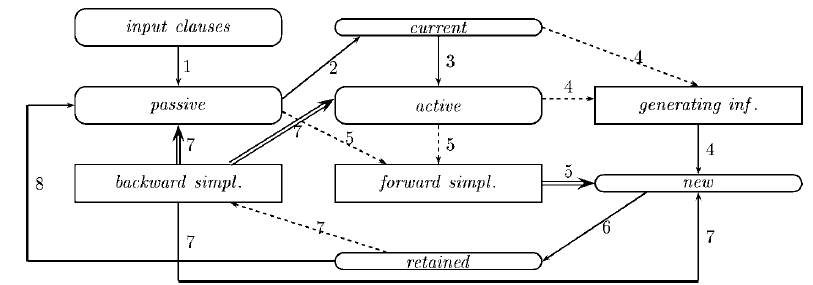
\includegraphics[width=\columnwidth]{figures/otter.png}
        \caption{Algoritmo otter \cite{riazanov2002design}}
    \end{figure}
    In aggiunta all'algoritmo precedente, ci sono:
    \begin{itemize}
        \item \emph{forward simplification}: un'operazione che cerca di semplificare la clausola \emph{new} coinvolgendo anche 
        le clausole negli insiemi \emph{active} e \emph{passive}.
        \item \emph{retained}: un insieme in cui passa la clausola \emph{new} dopo la \emph{forward simplification}. Su questa clausola viene effettuato un 
        \emph{retention test} e, tramite alcuni criteri (p.e. peso della clausola ovvero grandezza) e l'applicazione di \emph{deletion rules}, viene deciso se la clausola 
        è scartabile o no.
        \item \emph{backward simplification}: un'operazione eseguita dopo che la clausola ha superato il \emph{retention test}. In questo caso, al contrario della \emph{forward simplification}, 
        si cerca di semplificare gli insiemi \emph{active} e \emph{passive} tramite la clausola generata.
    \end{itemize}
    \item[\emph{Limited resource strategy}:] L'algoritmo \emph{lrs} è una variante di \emph{otter} poiché, aggiungendo un limite di tempo,
    cerca di identificare quali clausole nell'insieme \emph{passive} non hanno possibilità di essere selezionate e le scarta.
    \item[\emph{Discount}:] L'algoritmo \emph{discount} non usa l'insieme \emph{passive} per effettuare semplificazioni. Questa scelta è dettata dalla cardinalità di \emph{passive} in quanto è molto maggiore di \emph{active},
    quindi la velocità di inferenza potrebbe rallentare significativamente a causa delle semplificazioni sull'insieme \emph{passive}. 
\end{description}

Il \emph{kernel} è costituito da molte parti, le principali sono:
\begin{itemize}
    \item il \emph{main loop}
    \item il \emph{generating inference engine}
    \item il \emph{simplifying inference engine}
    \item uno \emph{splitter}
\end{itemize}
Sono definite a corredo numerose strutture dati, come indici e buffer, per gestire le sostituzioni, le unificazioni, \dots
\begin{description}
    \item[Main loop:] Contiene il vero e proprio algoritmo per la risoluzione del problema.
    \item[Generating inference engine:] \'E il cuore delle \emph{generating inferences}, in quanto funge da database per queste inferenze ed è responsabile del 
    loro utilizzo.
    \item[Simplifying inference engine:] \'E simile al precedente ma gestisce le inferenze che permettono le semplificazioni.
    \item[Splitter:] \'E un componente che interviene sulle clausole generate, che passano il \emph{retention test}, se sono \emph{splittable} ovvero
    \begin{definition}
        Siano $C_1,\dots C_n$ clausole, con $n\geq 2$, definite su insiemi disgiunti di variabili, 
        $F=C_1 \lor \dots \lor C_n$ è detta \emph{splittable} poiché è possibile dividerla in $n$ componenti $F_1=C_1, \dots, F_n=C_n$.
    \end{definition}
    Per rendere più efficiente questa operazione, lo \emph{splitter} collabora con un SAT solver (Minisat o Z3). Questa architettura è definita AVATAR \cite{voronkov2014avatar}. 
    \begin{figure}[H]
        \centering
        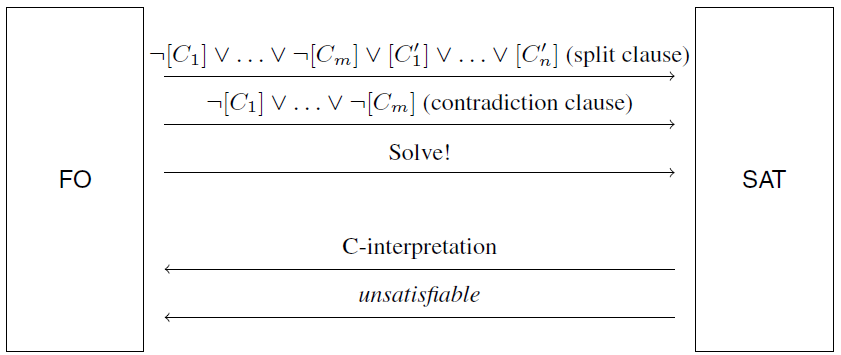
\includegraphics[width=\columnwidth]{figures/avatar.png}
        \caption{Collaborazione tra \textsc{Vampire} (FO) e SAT solver \cite{voronkov2014avatar}}
    \end{figure}
\end{description}

Il \emph{main loop}, prima di essere avviato, viene configurato tramite la scelta del tipo di algoritmo di saturazione da usare (lrs, otter o discount). 
Vengono inizializzati un \emph{generating inference engine} e un \emph{simplifying inference engine}, 
che vengono popolati rispettivamente con delle \emph{generating inferences} e delle \emph{simplifying inferences}.
Successivamente questi due \emph{engines} vengono collegati all'algoritmo di saturazione. A questo punto, 
il \emph{main loop} è configurato correttamente e può essere avviato. Nella figure sottostanti \ref{fig:kernelclass}, \ref{fig:genengineclass} e \ref{fig:simengineclass}, vengono presentate 
le relazioni tra le classi principali del kernel e le relazioni tra le classi dell'\emph{inference engine}.
\begin{figure}[H]
    \centering
    \begin{tikzpicture}
        \begin{class}[text width=7cm]{MainLoop}{5,1}
            \operation{+ run() : MainLoopResult}
            \operation{+ createFromOptions(prb : Problem\&, opt : Options\&) : MainLoop}
        \end{class}
        \begin{class}[text width=11cm]{SaturationAlgorithm}{0,-3}
            \inherit{MainLoop}
            \attribute{- generator : SimplifyingGeneratingInference}
            \attribute{- simplifier : ImmediateSimplificationEngine}
            \attribute{- splitter : Splitter*}
            \operation[0]{\# init() : void}
            \operation[0]{\# runImpl() : void}
            \operation{+ setGeneratingInferenceEngine(generator : \\SimplifyingGeneratingInference) : void}
            \operation{+ setImmediateSimplificationEngine(immediateSimplifier : \\ImmediateSimplificationEngine) : void}
        \end{class}
        \begin{class}[text width=3cm]{LRS}{-5,-10}
            \inherit{SaturationAlgorithm}
        \end{class}
        \begin{class}[text width=3cm]{Otter}{0,-10}
            \inherit{SaturationAlgorithm}
        \end{class}
        \begin{class}[text width=3cm]{Discount}{5,-10}
            \inherit{SaturationAlgorithm}
        \end{class}
        \begin{abstractclass}[text width=6cm]{SimplifyingGeneratingInference}{-5,-13}
        \end{abstractclass}
        \begin{abstractclass}[text width=6cm]{ImmediateSimplificationEngine}{5,-13}
        \end{abstractclass}
        \begin{class}[text width=5cm]{Splitter}{-5,0}
            \attribute{- sa : SaturationAlgorithm}
        \end{class}
        
        \association{SaturationAlgorithm}{}{}{SimplifyingGeneratingInference}{}{}
        \association{SaturationAlgorithm}{}{}{ImmediateSimplificationEngine}{}{}
        \association{SaturationAlgorithm}{}{}{Splitter}{}{}
    \end{tikzpicture}
    \caption{Relazioni tra le classi principali del \emph{kernel}}
    \label{fig:kernelclass}
\end{figure}

\begin{figure}[H]
    \begin{tikzpicture}[scale=0.7]
        \begin{abstractclass}[text width=6.5cm]{InferenceEngine}{0,0}
            \attribute{\# salg : SaturationAlgorithm*}
            \operation[0]{+ attach(salg : SaturationAlgorithm*) : void}
            \operation[0]{+ detach() : void}
        \end{abstractclass}
        \begin{abstractclass}[text width=6.5cm]{SimplifyingGeneratingInference}{0,-7}
            \inherit{InferenceEngine}
            \operation[0]{+ generateSimplify(premise : Clause*) : ClauseGenerationResult}
        \end{abstractclass}
        \begin{class}[text width=7cm]{GeneratingInferenceEngine}{5,-12.5}
            \inherit{SimplifyingGeneratingInference}
            \operation{+ generateSimplify(premise : Clause*) : ClauseGenerationResult}
            \operation[0]{+ generateClauses(Clause* premise) : ClauseIterator}
        \end{class}
        \begin{class}[text width=7cm]{CompositeGIE}{5,-18.5}
            \inherit{GeneratingInferenceEngine}
            \attribute{- inners : GIList*}
            \operation{+ addFront(fse : GeneratingInferenceEngine*) : void}
            \operation{+ generateClause(cl : Clause*) : Clause}
            \operation{+ attach(salg : SaturationAlgorithm*) : void}
            \operation{+ detach() : void}
        \end{class}
        \begin{class}[text width=7.5cm]{CompositeSGI}{-7,-12.5}
            \inherit{SimplifyingGeneratingInference}
            \attribute{- simplifiers : Stack$<$SimplifyingGeneratingInference*$>$}
            \attribute{- generators : Stack$<$GeneratingInferenceEngine*$>$}
            \operation{+ push(SimplifyingGeneratingInference*) : void}
            \operation{+ push(GeneratingInferenceEngine*) : void}
            \operation{+ generateSimplify(premise : Clause*) : ClauseGenerationResult}
            \operation{+ attach(salg : SaturationAlgorithm*) : void}
            \operation{+ detach() : void}
        \end{class}
    \end{tikzpicture}
    \caption{Relazioni tra le classi dell'\emph{inference engine} per le \emph{generating inferences}}
    \label{fig:genengineclass}
\end{figure}
\begin{figure}[H]
    \centering
    \begin{tikzpicture}
        \begin{abstractclass}[text width=6.5cm]{InferenceEngine}{0,0}
            \attribute{\# salg : SaturationAlgorithm*}
            \operation[0]{+ attach(salg : SaturationAlgorithm*) : void}
            \operation[0]{+ detach() : void}
        \end{abstractclass}
        \begin{abstractclass}[text width=6cm]{ImmediateSimplificationEngine}{0,-5}
            \inherit{InferenceEngine}
            \operation[0]{+ simplify(cl : Clause*) : Clause*}
        \end{abstractclass}
        \begin{class}[text width=7cm]{CompositeISE}{0,-8.5}
            \inherit{ImmediateSimplificationEngine}
            \attribute{- inners : ISList*}
            \operation{+ addFront(fse : ImmediateSimplificationEngine*) : void}
            \operation{+ simplify(cl : Clause*) : Clause}
            \operation{+ attach(salg : SaturationAlgorithm*) : void}
            \operation{+ detach() : void}
        \end{class}
    \end{tikzpicture}
    \caption{Relazioni tra le classi dell'\emph{inference engine} per le \emph{simplifying inferences}}
    \label{fig:simengineclass}
\end{figure}
Si noti che tutte le \emph{generating inferences} (resolution, superposition) ereditano la classe \verb|GeneratingInferenceEngine|,
così come tutte le \emph{simplifying inferences} ereditano la classe \verb|ImmediateSimplificationEngine|.

Nella fase di configurazione del \emph{main loop}, viene inizializzato un \verb|CompositeGIE| in cui 
vengono memorizzate tutte le inferenze tramite la funzione \verb|addFront()| nella lista \emph{inners}.
Una volta aggiunte tutte le regole di inferenza, viene inizializzato un \verb|CompositeSGI| che memorizza
il \verb|CompositeGIE| nello stack \emph{generators} e altre regole di semplificazione nello stack \emph{simplifiers}.
Nello stesso modo viene inizializzato un \verb|CompositeISE|. Alla fine, al \verb|SaturationAlgorithm| viene assegnato un generatore (ovvero il \verb|CompositeGIE|)
tramite la funzione \verb|setGeneratingInferenceEngine()| e un \verb|ImmediateSimplificationEngine| tramite la funzione 
apposita. 
\clearpage
\begin{example}
    Di seguito viene riportato un algoritmo riassuntivo, definendo un algoritmo di saturazione di tipo \emph{otter} con un \emph{superposition inference system} come visto 
nella definizione \ref{supdef}:
\begin{algorithm}
    \caption{Esempio semplificato di configurazione di un algoritmo di saturazione in \textsc{Vampire}}
    \begin{algorithmic}
        \State \textbf{var} salg : \verb|SaturationAlgorithm|
        \State \textbf{var} gie : \verb|CompositeGIE|
        \State \textbf{var} sgi : \verb|CompositeSGI|
        \Function{createFromOptions}{}    
        \State salg = \verb|Otter|
        \State gie.\emph{addFront}(\verb|Resolution|)
        \State gie.\emph{addFront}(\verb|Factoring|)
        \State gie.\emph{addFront}(\verb|Superposition|)
        \State gie.\emph{addFront}(\verb|EqualityResolution|)
        \State gie.\emph{addFront}(\verb|EqualityFactoring|)

        \State sgi.\emph{push}(gie)
        \State salg.\emph{setGeneratingInferenceEngine}(sgi)
        \State salg.\emph{setImmediateSimplificationEngine}(\emph{createISE}())
        \State \textbf{return} salg
        \EndFunction
    \end{algorithmic}
\end{algorithm}
\end{example}
La trattazione è stata limitata a una semplificazione di \textsc{Vampire}, al fine di fornire una base 
per la comprensione dei concetti che verranno affrontati nei capitoli successivi. 

